% Created 2016-05-27 Fri 17:19
\documentclass[presentation]{beamer}
\usepackage[utf8]{inputenc}
\usepackage[T1]{fontenc}
\usepackage{fixltx2e}
\usepackage{graphicx}
\usepackage{longtable}
\usepackage{float}
\usepackage{wrapfig}
\usepackage{rotating}
\usepackage[normalem]{ulem}
\usepackage{amsmath}
\usepackage{textcomp}
\usepackage{marvosym}
\usepackage{wasysym}
\usepackage{amssymb}
\usepackage{hyperref}
\tolerance=1000
\usepackage{minted}
\usepackage[utf8]{inputenc}
\usepackage{color}
\usetheme[height=7mm]{Rochester}
\setbeamertemplate{footline}[frame number]
\usecolortheme[accent=red, light]{solarized}
\setbeamercolor{frametitle}{bg=solarizedRebase02,fg=solarizedAccent}
\setbeamercolor{author in head/foot}{bg=solarizedRebase02,fg=solarizedRebase01}
\setbeamercolor{title in head/foot}{bg=solarizedRebase02,fg=solarizedRebase01}
\setbeamercolor{block title}{bg=solarizedRebase0,fg=solarizedRebase02}
\setbeamercolor{block body}{bg=solarizedRebase02,fg=solarizedRebase0}
\setbeamercolor{item}{bg=solarizedRebase02,fg=solarizedAccent}
\beamertemplatenavigationsymbolsempty
\usemintedstyle{manni}
\AtBeginSection[]{
\begin{frame}
\vfill
\centering
\begin{beamercolorbox}[sep=8pt,center,shadow=true,rounded=true]{title}
\Huge\insertsectionhead\par%
\end{beamercolorbox}
\vfill
\end{frame}
}
\usetheme{default}
\author{Sebastian Stabinger, Simon Hangl}
\date{\today}
\title{Exceptions}
\hypersetup{
  pdfkeywords={},
  pdfsubject={},
  pdfcreator={Emacs 24.4.1 (Org mode 8.2.10)}}
\begin{document}

\maketitle

\section{Problem}
\label{sec-1}
\begin{frame}[fragile,label=sec-1-1]{Fehlerbehandlung (1)}
\begin{block}{Was ist das?}
	\begin{itemize}
		\item In \emph{JEDEM} Programm treten Fehler auf
		\begin{itemize}
			\item Sogar in euren Programmen ;)
		\end{itemize}
		\item Passieren unregelmäßig
		\begin{itemize}
			\item Nicht jeder Fehler muss bei jeder Ausführung auftreten
		\end{itemize}
		\item Ein stabiles Programm muss diese Fehler sinnvoll abarbeiten
		\item Bisher wurden die meisten Fehler ignoriert
		\begin{itemize}
			\item I/O Fehler
			\item Speicherzugriffsfehler
			\item Bad alloc
		\end{itemize}
	\end{itemize}
\end{block}

\end{frame}

\begin{frame}[fragile,label=sec-1-1]{Fehlerbehandlung (2)}
\begin{block}{Warum ist das wichtig?}
	\begin{itemize}
		\item In großen system kann Fehlerbehandlungscode bis zu 80 Prozent ausmachen
		\item Qualität eines Programmes hängt zu einem großen Teil von der Stabilität ab
		\begin{itemize}
			\item Programm sollte nicht laufend abstürzen
		\end{itemize}
		\item Wahl des Fehlerbehandlungsmechanismus bestimmt, wieviel Zeit investiert werden muss
	\end{itemize}
\end{block}

\end{frame}

\begin{frame}[fragile,label=sec-1-1]{Fehlerbehandlung in C}
\begin{block}{Schwierige Fehlerbehandlung}
\begin{itemize}
	\item Sehr oft Detailwissen zu den verwendeten Funktionen notwendig
	\begin{itemize}
		\item z.B. Fehlercodes
	\end{itemize}
	\item Wiederholungen notwendig
\end{itemize}
\end{block}
\begin{exampleblock}{Beispiel}
\begin{minted}[fontsize=\scriptsize,numberblanklines=false]{c++}
#include <stdlib.h>

int main() {
	// speicher allockieren
	int* arr = (int*) malloc(10 * sizeof(int));
	if(!arr) {
		// fehlerbehandlung!!!
	}
	// ...
	// dieselbe fehlerbehandlung bei jedem malloc notwendig
	return EXIT_SUCCESS;
}
\end{minted}
\end{exampleblock}
\end{frame}

\begin{frame}[fragile,label=sec-1-1]{Fehlerbehandlung in C++}
\begin{block}{Exceptions}
\begin{itemize}
	\item C++ bietet Update auf moderene Fehlerbehandlungsmechanismen
	\item Exceptions (Ausnahmefälle)
\end{itemize}
\end{block}
\begin{exampleblock}{Beispiel}
\begin{minted}[fontsize=\scriptsize,numberblanklines=false]{c++}
int main() {
  try {
    // probiere folgenden code
    while (true)
      new int[100000000ul];
    // "fange" folgenden ausnahmefall
    } catch (const std::bad_alloc& e) {
      // fehlerbehandlung
      std::cout << "Allocation failed: " << e.what() << '\n';
    }
}
\end{minted}
\end{exampleblock}

\end{frame}

\begin{frame}[fragile,label=sec-1-1]{Exceptions}
\begin{block}{Was ist das?}
\begin{enumerate}
	\item Ausnahmefälle treten in einem Block auf
	\item Exception wird "geworfen"
	\item Exception reißt das Programm solange mit, bis sie "gefangen" wird
	\begin{itemize}
		\item Wird die Exception nicht gefangen, kommt es zum Programmabsturz
	\end{itemize}
\end{enumerate}
\end{block}

\end{frame}

\begin{frame}[fragile,label=sec-1-1]{Fangen von Exceptions}
\begin{exampleblock}{Syntax}
\begin{minted}[fontsize=\scriptsize,numberblanklines=false]{c++}
int main() {
  try {
    // protected code
  } catch( ExceptionType e1 ) {
    // catch block
  } catch( ExceptionType e2 ) {
    // catch block
  } catch( ExceptionType eN ) {
    // catch block
  }
}
\end{minted}
\end{exampleblock}

\end{frame}

\begin{frame}[fragile,label=sec-1-1]{Arten von Exceptions}
\begin{block}{Arten}
\begin{itemize}
	\item Prinzipiell kann (fast) jedes Objekt geworfen werden
	\item Exception Standardtypen
	\item Benutzerdefinierte Exceptiontypen
\end{itemize}
\end{block}

\end{frame}

\begin{frame}[fragile,label=sec-1-1]{Arten von Exceptions}
\begin{exampleblock}{Werfen eines beliebigen Objekts}
\begin{minted}[fontsize=\scriptsize,numberblanklines=false]{c++}
double division(int a, int b) {
  if(b == 0)
    throw "Division by zero";
  return a / b;
}
int main() {
  int x = 50;
  int y = 0;
  double z = 0;
  try {
    z = division(x, y);
    cout << z << endl;
  } catch (const char* msg) {
    cerr << msg << endl;
  }
  return EXIT_SUCCESS;
}
\end{minted}
\end{exampleblock}

\end{frame}

\begin{frame}[fragile,label=sec-1-1]{Arten von Exceptions}
\begin{block}{Exception Standardtypen}
	\centering
	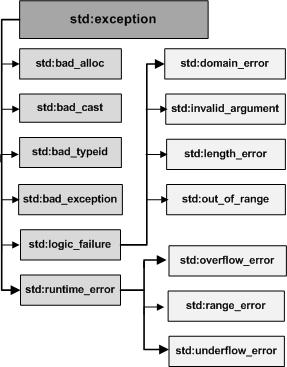
\includegraphics[width=0.5\textwidth]{img/exceptions.jpg}
\end{block}

\end{frame}

\begin{frame}[fragile,label=sec-1-1]{Arten von Exceptions}
\begin{exampleblock}{Benutzerdefinierte Exceptiontypen}
\begin{minted}[fontsize=\scriptsize,numberblanklines=false]{c++}
#include <exception>
class BadUserException : public exception {
  const char * what () const throw () {
    return "my own exception message";
  }
};
int main() {
  try {
    throw BadUserException();
  } catch(BadUserException& e) {
    std::cout << "bad user" << std::endl;
    std::cout << e.what() << std::endl;
  } catch(std::exception& e) {
	// handle other errors
  }
}
\end{minted}
\end{exampleblock}

\end{frame}

\end{document}